\documentclass[11pt]{article}
\usepackage[margin=0.5in, top=0.4in, bottom=0.6in]{geometry}
\usepackage{amsmath, amssymb}
\usepackage{graphicx}
\usepackage{hyperref}
\usepackage{booktabs}
\usepackage{parskip}
\usepackage{titlesec}
\usepackage{enumitem}
\usepackage[numbers]{natbib}
\usepackage{tikz}
\usetikzlibrary{positioning}

% Reduce spacing around sections and subsections
\titlespacing*{\section}{0pt}{4pt}{2pt}
\titlespacing*{\subsection}{0pt}{3pt}{1pt}

% Reduce spacing for list environments globally
\setlist{nosep, topsep=0pt, partopsep=0pt, parsep=0pt, itemsep=0pt}

% Reduce spacing between paragraphs
\setlength{\parskip}{2pt}

\hypersetup{
colorlinks=true,
linkcolor=black,
citecolor=black,
urlcolor=black
}

\title{
\vspace{-2.5em}
\textbf{Beyond Pattern Matching: Causal Concept Representations for Strategic Decision-Making in Chess}
\vspace{-1em}
}

\author{
Abdulla Alfalasi \quad Mohammmed AlBalooshi \\
\small ML808 --- Causality \& Machine Learning \\
\small Mohamed Bin Zayed University of AI
}

\date{Submitted: 27 March 2026}

\begin{document}
\maketitle
\vspace{-2.5em}

% -------------------------------------------------------
\section*{Key Project Idea}
% -------------------------------------------------------

This project investigates whether human-interpretable, causally motivated concepts can serve as a reusable abstraction that enables data-efficient estimation of intervention effects in strategic decision-making.\cite{scholkopf2021towards,pearl2009causality} Instead of operating directly on high-dimensional state spaces (e.g., raw chess boards) that entangle many factors, we propose to work in a concept space that encodes meaningful mechanisms such as piece activity, king safety, pawn structure, material balance, and space control, derived from a strong chess engine.\cite{lemeire2005causalmodelsinchess,stockfish} In a chess domain where both raw board states and expert-defined concepts are available, we systematically compare how different representations affect the accuracy, robustness, and sample efficiency of treatment effect estimation for strategic interventions (e.g., adopting an aggressive vs.\ conservative strategy).\cite{chernozhukov2018double,scholkopf2021towards} Our overarching aim is to test the hypothesis that once an appropriate concept basis is fixed, estimating the consequences of new interventions requires substantially less data than in purely statistical pattern-matching regimes.\cite{lake2017building,scholkopf2021towards}

Concretely, we focus on two main hypotheses: (H1) that concept-level representations reduce the number of samples required to achieve a target ATE estimation error compared to raw board encodings and a learned latent representation, and (H2) that concept-level representations yield more stable ATE estimates under changes in nuisance model classes used within a doubly robust estimation pipeline.

% -------------------------------------------------------
\section*{Causal Perspective}
% -------------------------------------------------------

We frame the problem in terms of interventional queries rather than observational prediction.\cite{pearl2009causality} The central object is the interventional distribution \(P(Y \mid do(T))\), where the treatment \(T\) denotes a player's strategic choice (e.g., aggressive vs.\ conservative) and the outcome \(Y\) is a semi-synthetic payoff constructed from game trajectories with a planted ground-truth treatment effect.\cite{hill2011bayesian} We explicitly construct a structural causal model (SCM) over raw board states, expert concepts, opponent and player strength, strategic choices, and payoffs, and use it to define the Average Treatment Effect (ATE) as
\[
\text{ATE} = \mathbb{E}[Y \mid do(T=1)] - \mathbb{E}[Y \mid do(T=0)].
\]
Within this SCM, concept vectors are treated as a causal abstraction of the raw state: a deterministic map from board configurations to concept features that is intended to retain all variables necessary for valid adjustment under the back-door criterion.\cite{pearl2009causality,scholkopf2021towards} We study when concept-level covariates are sufficient for identifying the ATE, how they affect overlap and model misspecification sensitivity in doubly robust estimation, and how their use changes the amount of data required to accurately estimate interventional quantities across different confounding regimes and payoff definitions.\cite{chernozhukov2018double,kuang2020information,deconfoundingScores}

To isolate the role of representation, we compare three covariate spaces within the same SCM: (i) a high-dimensional raw board encoding, (ii) an expert-defined concept vector, and (iii) a learned low-dimensional representation inspired by information-bottleneck and deconfounding approaches to treatment-effect estimation.\cite{kuang2020information,deconfoundingScores}

% -------------------------------------------------------
\section*{Motivations}
% -------------------------------------------------------

Modern AI systems often rely on large-scale statistical pattern matching, which yields impressive predictive performance but requires vast amounts of data and struggles with counterfactual and ``what-if'' reasoning.\cite{lake2017building,reasoningAIMag} In contrast, human decision-making appears to rely on compact libraries of concepts and causal relations, enabling rapid adaptation to new tasks and environments once core concepts are in place.\cite{lake2017building,towardHumanLevelConcept} Causal representation learning and concept bottleneck models suggest that aligning representations with underlying causal structure can improve robustness and interpretability, but there is limited empirical evidence on when interpretable, expert-defined concepts actually improve causal effect estimation and reduce data requirements.\cite{scholkopf2021towards,koh2020concept,fromCausalToConcept} Strategic games like chess offer a unique testbed: they provide rich, high-dimensional raw states, well-understood expert concepts, and controlled environments for defining interventions and payoffs, and they have been used before to study causal models and the evaluation of patterns in a principled way.\cite{lemeire2005causalmodelsinchess,fortressesPaper,causalMaskingSpatial} By rigorously comparing raw, concept-based, and learned representations in this setting, we aim to quantify how far causal, concept-level abstractions can move us away from brute-force pattern matching toward data-efficient causal reasoning in a realistic strategic domain.\cite{scholkopf2021towards,causalReasoningRL,fromCausalToConcept}

Unlike structural causal bottleneck models and causally reliable concept bottleneck models, which learn their bottleneck representations end-to-end, we treat the concept map as a fixed, expert-defined abstraction and use chess as a controlled testbed to study when such interpretable abstractions empirically improve treatment-effect estimation and sample efficiency.\cite{fromCausalToConcept,scholkopf2021towards}

% -------------------------------------------------------
\section*{Contributions}
% -------------------------------------------------------

\begin{enumerate}
\item We formalize a structural causal model for strategic decision-making in chess that links raw board states, expert-defined concept abstractions, opponent and player strength, strategic feasibility, and semi-synthetic payoffs, explicitly characterizing conditions under which concept-level covariates, together with exogenous skill variables, can satisfy the back-door criterion for ATE identification.\cite{pearl2009causality,lemeire2005causalmodelsinchess}
\item We design a semi-synthetic experimental framework in which confounding structure and strength can be systematically varied---via explicit potential outcome models and latent-confounder stress tests---enabling controlled evaluation of representation choices (raw boards, expert concepts, and a learned embedding) on both bias and variance of treatment effect estimators.\cite{hill2011bayesian,kuang2020information,deconfoundingScores}
\item We empirically demonstrate how concept-based representations affect sample efficiency for interventional inference by measuring ATE estimation error as a function of training set size across the three representations, and by comparing robustness to nuisance-model misspecification under a doubly robust estimator and a simpler baseline.\cite{chernozhukov2018double,kuang2020information,scholkopf2021towards}
\item We illustrate how concept-level causal abstractions can support simple ``what-if'' queries about strategic interventions---such as manipulating specific concepts (e.g., king safety) while holding others (e.g., material balance) fixed---providing evidence that such representations bring AI systems a step closer to conceptual, causal reasoning in a realistic strategic domain and connect naturally to prior work on causal models for evaluating chess patterns and spatial representations in chess agents.\cite{lemeire2005causalmodelsinchess,fortressesPaper,causalMaskingSpatial}
\end{enumerate}

% -------------------------------------------------------
\section*{Structural Causal Model}
% -------------------------------------------------------

\subsection*{Variables and Structural Assumptions}

We work at the level of individual decision points within games. For each decision, we define the following variables:

\begin{itemize}
\item \(S\): \emph{Raw board state}. A high-dimensional encoding of the pre-move position, including piece locations, side to move, castling rights, and other rule-relevant information. This is treated as the underlying spatial state of the game.
\item \(C = f(S)\): \emph{Concept-level representation}. A low-dimensional vector of expert-defined chess concepts (e.g., king safety, material balance, piece activity, pawn structure, space control), obtained via a fixed evaluation function implemented by a strong chess engine.\cite{lemeire2005causalmodelsinchess,stockfish}
\item \(X\): \emph{Pre-treatment player/opponent context}. A set of exogenous and meta-variables such as player and opponent Elo, color, time control, clock features, game phase, and opening code. These variables may influence both strategic choices and outcomes but are not deterministically derived from \(S\).
\item \(F\): \emph{Feasibility indicator}. A binary variable indicating whether the actually played move lies within a high-quality candidate set (e.g., top-\(k\) engine moves) at state \(S\). All causal estimands are defined conditional on \(F=1\).
\item \(T\): \emph{Treatment (strategy choice)}. A binary indicator of the player's strategic decision at the position, e.g., \(T=1\) for an ``aggressive'' move and \(T=0\) for a ``conservative'' move, defined by a rule-based labeling of moves using non-evaluative features (captures, checks, king-zone pressure, etc.).
\item \(Y\): \emph{Outcome}. A semi-synthetic payoff anchored in engine evaluations and augmented via an explicit potential-outcomes model, with a planted ground-truth average treatment effect. This allows direct measurement of estimation bias.
\item \(U\): \emph{Latent factors}. Unobserved variables (e.g., short-term psychological factors, latent style) that may influence both \(T\) and \(Y\). These are used in sensitivity analyses but are not available for adjustment.
\end{itemize}

We consider alternative observed adjustment sets constructed from these variables:
\[
X_{\text{raw}} = (S, X), \qquad
X_{\text{concept}} = (C, X), \qquad
X_{\text{learned}} = (Z, X),
\]
where \(Z = g(S, X)\) is a learned representation (e.g., information-bottleneck or deconfounding embedding) trained to preserve information relevant for treatment effect estimation.\cite{kuang2020information,deconfoundingScores}

\subsection*{DAG and Causal Structure}

The qualitative causal structure of the decision problem is summarized by the directed acyclic graph:
\[
X \rightarrow S, \quad X \rightarrow T, \quad X \rightarrow Y,
\]
\[
S \rightarrow T, \quad S \rightarrow Y, \quad T \rightarrow Y,
\]
with an additional latent parent \(U\) influencing both \(T\) and \(Y\):
\[
U \rightarrow T, \quad U \rightarrow Y,
\]
and all edges understood to be restricted to the feasible-decision population \(F=1\).
The concept vector \(C = f(S)\) does not appear as a separate node in this graph;
it is a deterministic encoding of \(S\) and introduces no new causal ancestry beyond
what is already present through \(S\). We instead treat \(C\) as an alternative
covariate encoding for the adjustment set: rather than conditioning on \(S\) directly,
one may condition on \(f(S)\) instead, and the three adjustment sets
\(X_{\text{raw}}\), \(X_{\text{concept}}\), and \(X_{\text{learned}}\) represent
three such encoding choices for the same underlying adjustment problem.
The edge \(X \rightarrow S\) reflects a selection mechanism rather than a direct
physical cause: players with different Elo, styles, or opening preferences
systematically reach different board positions, inducing a statistical dependence
between \(X\) and \(S\) in the observational distribution.

Intuitively, pre-treatment context \(X\) shapes both the raw state \(S\) (through opening choices, game phase, and time control) and the player's strategic tendencies, and it directly affects the difficulty of the position and thus the outcome. The raw spatial state \(S\), together with \(X\), informs the set of plausible moves and the eventual strategy choice \(T\), while \(T\) exerts a direct causal effect on the outcome through the chosen move.

Within this SCM, the target causal estimand is the conditional ATE among feasible decisions:
\[
\tau = \mathbb{E}[Y(1) - Y(0) \mid F = 1],
\]
where \(Y(1)\) and \(Y(0)\) denote potential outcomes under aggressive and conservative strategies, respectively. Identification of \(\tau\) from observational data requires a version of conditional exchangeability,
\[
(Y(0), Y(1)) \perp T \,\mid\, X_{\text{adj}},\, F=1,
\]
for some choice of adjustment set \(X_{\text{adj}}\), together with positivity and consistency.\cite{pearl2009causality,hill2011bayesian}

We do not assume that any candidate adjustment set is perfectly valid in practice. Instead, we treat
\[
X_{\text{adj}} \in \{ X_{\text{raw}},\, X_{\text{concept}},\, X_{\text{learned}} \}
\]
as competing approximations to a valid back-door adjustment set and empirically compare how close each comes to satisfying the requisite ignorability condition, as measured by ATE bias, variance, and sample-efficiency behavior under the semi-synthetic data-generating process.

\subsection*{Role of Concept-Level Abstraction}

Concept vectors \(C = f(S)\) are a fixed, deterministic encoding of the raw state
\(S\), not a separate causal parent of \(T\) or \(Y\). Since all information in \(C\)
is already contained in \(S\), the adjustment set \((C, X)\) does not block any
back-door paths that \((S, X)\) does not already block---but it may approximate
the true confounding structure more efficiently by discarding causally
irrelevant micro-structure in \(S\). Under the idealized assumption that \(C\) is
sufficient for the joint influence of \(S\) on \((T, Y)\), an adjustment set
involving \((C, X)\) would satisfy the back-door criterion whenever \((S, X)\) does.
Our experiments probe to what extent this ideal holds in practice, by comparing ATE
estimation performance when conditioning on \(X_{\text{raw}}\), \(X_{\text{concept}}\),
and \(X_{\text{learned}}\) across varying confounding structures and sample sizes.

\begin{figure}[t]
\centering
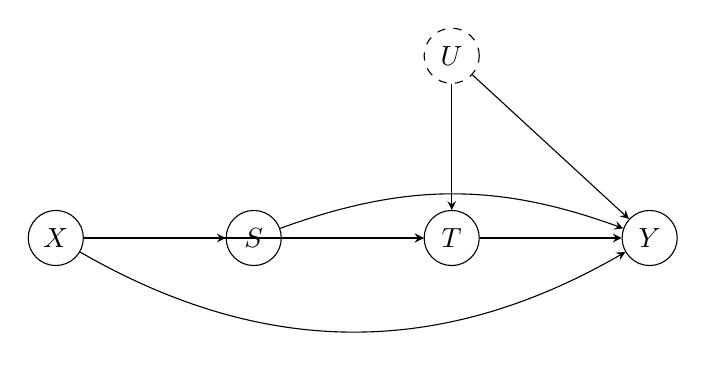
\begin{tikzpicture}[
  node distance=1.6cm and 1.8cm,
  roundnode/.style={circle, draw=black, minimum size=7mm, inner sep=0pt},
  latentnode/.style={circle, draw=black, dashed, minimum size=7mm, inner sep=0pt},
  >=stealth
]
  % Nodes
  \node[roundnode] (X) {$X$};
  \node[roundnode, right=of X] (S) {$S$};
  \node[roundnode, right=of S] (T) {$T$};
  \node[roundnode, right=of T] (Y) {$Y$};
  \node[latentnode, above=of T] (U) {$U$};

  % Edges from X
  \draw[->] (X) -- (S);
  \draw[->] (X) -- (T);
  \draw[->] (X) to[bend right=30] (Y);

  % Edges from S
  \draw[->] (S) -- (T);
  \draw[->] (S) to[bend left=20] (Y);

  % Treatment to outcome
  \draw[->] (T) -- (Y);

  % Latent U
  \draw[->] (U) -- (T);
  \draw[->] (U) -- (Y);
\end{tikzpicture}
\caption{Structural causal model for a single chess decision.
$X$ denotes pre-treatment player/opponent context (e.g., Elo, color, time control),
$S$ the raw board state, $T$ the strategic treatment (aggressive vs.\ conservative),
$Y$ the semi-synthetic payoff, and $U$ latent unobserved factors.
$C = f(S)$ is not a separate causal node: it is a deterministic encoding of $S$
used as an alternative covariate representation in the adjustment set.
We compare adjustment on $(S, X)$, $(f(S), X)$, and $(Z, X)$ to assess
how different encodings of state approximate a valid back-door adjustment set.}
\label{fig:scm_chess}
\end{figure}

% -------------------------------------------------------
\bibliographystyle{plain}
\bibliography{refs}

\end{document}